\section{Painel Administrativo}\label{RS0006:introducao}

\begin{displayquote}
    Muitas das informações contidas aqui podem ser complementadas no Guia de Estilos, principalmente no que se refere à inserção de imagens e informações estruturadas dentro das publicações.
\end{displayquote}

\subsection{Operação}

O Painel Administrativo pode ser acessado no mesmo endereço do Portal Institucional, adicionando-se a \gls{URI} definida na configuração do portal (ver Guias do Desenvolvedor e do Operador).

A primeira tela apresentada é a de autenticação do usuário (ver \cref{RS0006:fig:img001}). O Portal Institucional é de acesso público e irrestrito, e para acessá-lo não é necessário credencial alguma (e nenhuma é usada ou registrada durante a navegação pelo portal), porém o Painel Administrativo é de acesso restrito e pode ser até mesmo configurado pela operação de redes da instituição para não ser acessado externamente se desejado.

\begin{figure}[!ht]
    \centering
    \includegraphics[scale=.25]{img001}
    \caption{Tela de acesso ao Painel Administrativo}\label{RS0006:fig:img001}
\end{figure}

\subsubsection{Lista de Estruturas de Dados}

Este painel apresenta uma lista (ver \cref{RS0006:fig:img002}) de estruturas de dados definidas pelos desenvolvedores (ver Guia do Desenvolvedor).

\begin{figure}[!ht]
    \centering
    \includegraphics[scale=.25]{img002}
    \caption{Lista de estruturas de dados}\label{RS0006:fig:img002}
\end{figure}

Algumas das estruturas existentes é a própria lista de usuários do painel ou a lista de publicações (conteúdo dinâmico, ver \cref{RS0006:fig:img003}).

\begin{figure}[!ht]
    \centering
    \includegraphics[scale=.25]{img003}
    \caption{Lista de conteúdo de uma estrutura de dados}\label{RS0006:fig:img003}
\end{figure}

\subsubsection{Menu do Painel Administrativo}

O painel apresenta um menu (barra superior da página) com duas áreas de navegação (ver \cref{RS0006:fig:img003a} e \cref{RS0006:fig:img003b}).

\begin{figure}[!ht]
    \centering
    \includegraphics[scale=.25]{img003a}
    \caption{Menu de navegação esquerdo}\label{RS0006:fig:img003a}
\end{figure}

No menu esquerdo temos o botão para retornar à lista de estruturas e uma opção para editr a lista de usuários.

\begin{figure}[!ht]
    \centering
    \includegraphics[scale=.25]{img003b}
    \caption{Menu de navegação direito}\label{RS0006:fig:img003b}
\end{figure}

No menu direito temos a opção de selecionar um dos idiomas disponíveis e navegar para o próprio portal ou sair do painel.

A disponibilidade de idiomas pode ser configurada pelo desenvolvedor e a operação do portal (ver Guia do Desenvolvedor e Guia do Operador).

\subsubsection{Ordenação dos documentos}

É possível reordenar os documentos apresentados na lista usando a opção no topo da página (ver \cref{RS0006:fig:img003c})

\begin{figure}[!ht]
    \centering
    \includegraphics[scale=.25]{img003c}
    \caption{Ordenando a lista de documentos}\label{RS0006:fig:img003c}
\end{figure}

Podemos inverter a ordem segurando a tecla $\bm{g}$ ao escolher a coluna desejada.

\subsubsection{Filtrando documentos}

Podemos ainda filtrar documentos de acordo com critérios de seleção escolhendo uma das colunas (ver \cref{RS0006:fig:img003d}).

\begin{figure}[!ht]
    \centering
    \includegraphics[scale=.25]{img003d}
    \caption{Filtrando a lista de documentos}\label{RS0006:fig:img003d}
\end{figure}

Caso seja um atributo com valores particulares, várias opções podem ser selecionadas ao mesmo tempo pressionando-se a tecla $\bm{CTRL}$ no ``\textbf{Windows}'' ou $\bm{CMD}$ no ``\textbf{macOS}'' (ver \cref{RS0006:fig:img003e}).

\begin{figure}[!ht]
    \centering
    \includegraphics[scale=.25]{img003e}
    \caption{Selecionando valores de atributo com valores restritos}\label{RS0006:fig:img003e}
\end{figure}

\subsubsection{Localizando documentos}

Podemos localizar o documento usando a barra de pesquisa (ver \cref{RS0006:fig:img003f})

\begin{figure}[!ht]
    \centering
    \includegraphics[scale=.25]{img003f}
    \caption{Pesquisando documento}\label{RS0006:fig:img003f}
\end{figure}

O resultado final será uma lista bastante reduzida dos documentos que atendem os critérios aplicados (ver \cref{RS0006:fig:img003g}).

\begin{figure}[!ht]
    \centering
    \includegraphics[scale=.25]{img003g}
    \caption{Resultado da pesquisa}\label{RS0006:fig:img003g}
\end{figure}

\subsubsection{Criando documentos}

Para criar um documento, basta usar o botão no canto superior direito ``\textit{New ...}''\footnote{O texto será complementado com o tipo de documento que a lista estiver apresentando. No caso da lista ``\textit{Posts}'' será ``\textit{New Post}''.}

\begin{figure}[!ht]
    \centering
    \includegraphics[scale=.25]{img003h}
    \caption{Criando um novo documento}\label{RS0006:fig:img003h}
\end{figure}

Na \cref{RS0006:fig:img003h} vemos a tela de criação do documento. Atributos obrigatórios (ver Guida do Desenvolvedor) serão apresentados nesta tela (no exemplo, o ``Título'' da publicação e as ``Categorias'' - ao menos uma deve ser informada).

\subsubsection{Excluindo documentos}

O documento poderá ser excluído diretamente na lista (o ícone no formato de uma lata de lixo logo à esquerda de cada linha - ver \cref{RS0006:fig:img003g}).

Na página de edição do documento temos o botão ``\textit{delete ...}''\footnote{O texto será complementado com o tipo de documento que estiver apresentando. Para o document ``\textit{Post}'' será ``\textit{delete post}''.}

\begin{figure}[!ht]
    \centering
    \includegraphics[scale=.25]{img003i}
    \caption{Excluindo um novo documento}\label{RS0006:fig:img003i}
\end{figure}

Na \cref{RS0006:fig:img003i} vemos que o botão somente entra em destaque quando o cursor passa sobre ele.

\subsection{Estrutura de apresentação e permissões de publicação}

O Portal Institucional se subdivide em sete painéis principais (ver \cref{RS0006:fig:portal}). A ordenação ou inclusão ou exclusão de novos painéis pode facilmente ser feita por um desenvolvedor (ver Guia do Desenvolvedor).

\begin{figure}[!ht]
    \centering
    \fbox{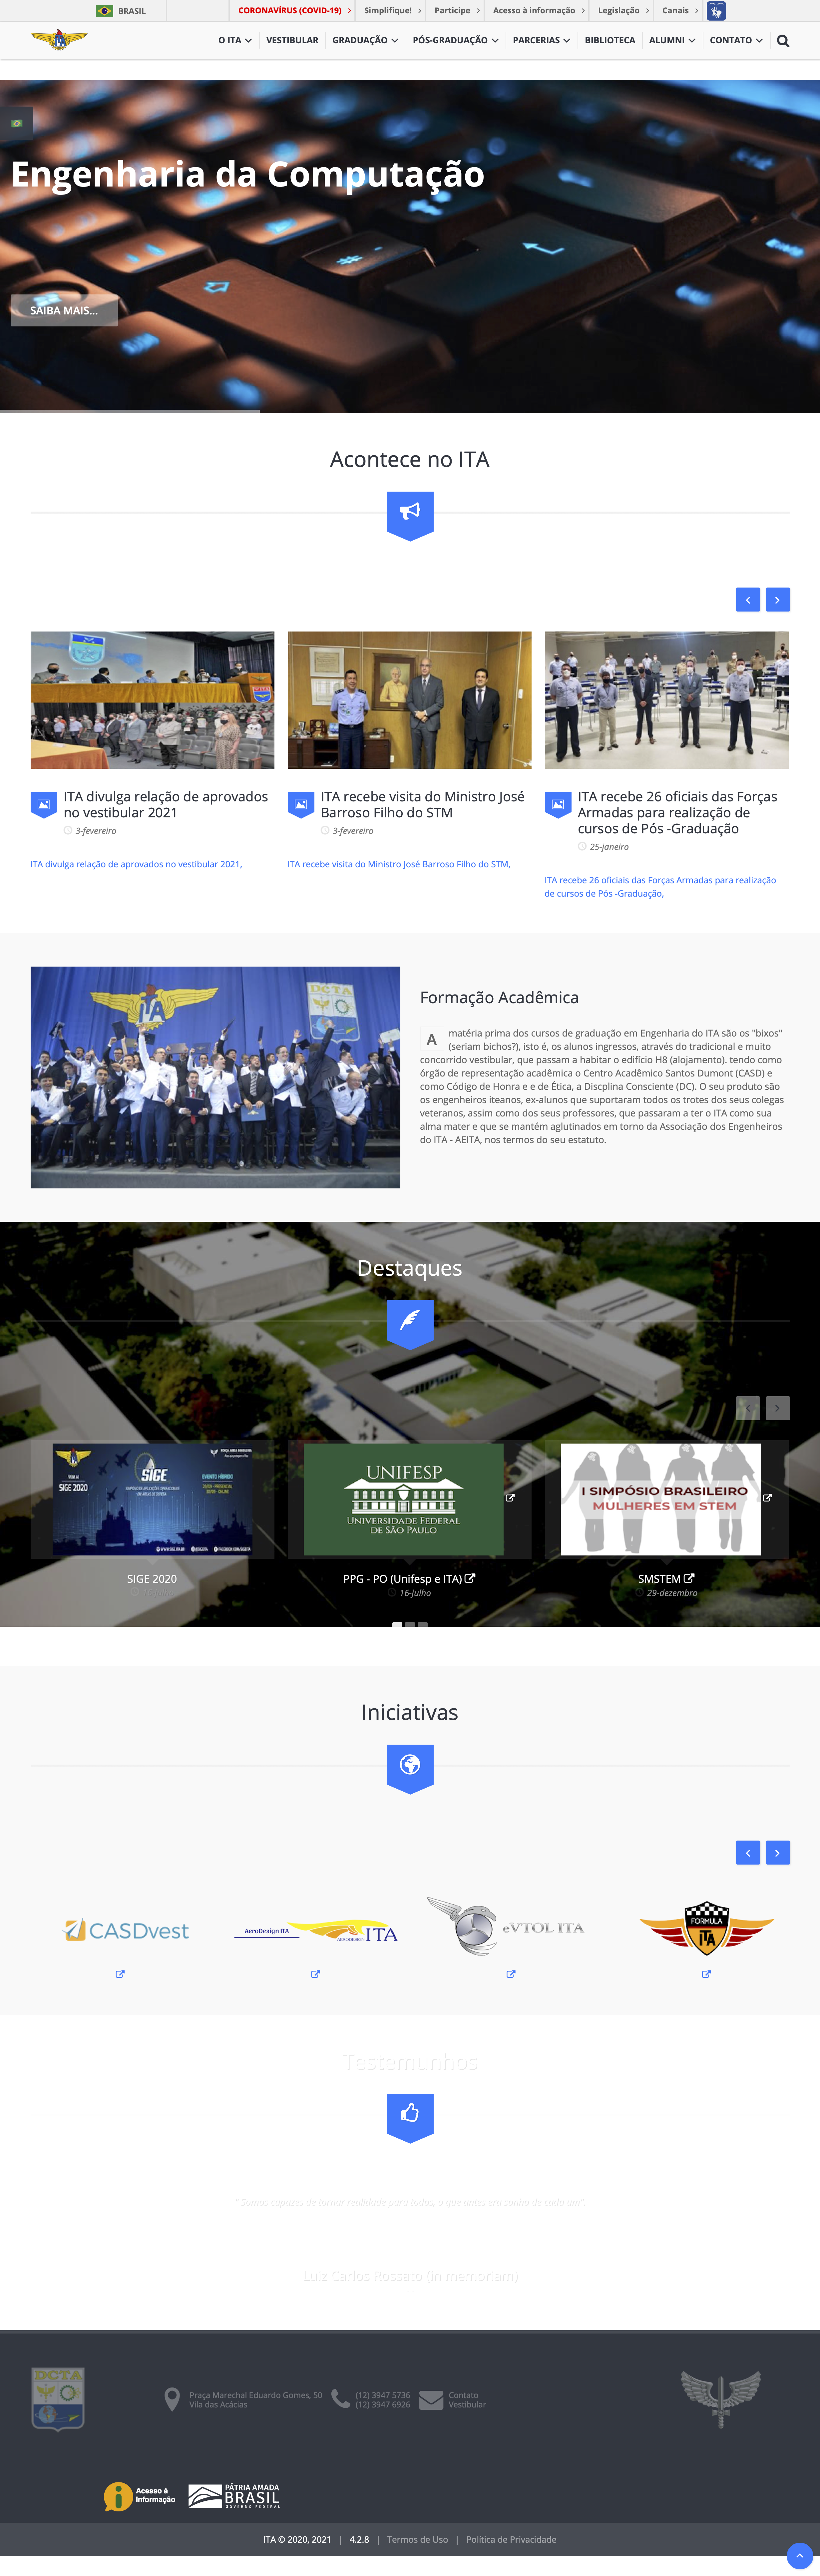
\includegraphics[scale=.075]{../anexos/portal}}
    \caption{Página principal do Portal Institucional}\label{RS0006:fig:portal}
\end{figure}

Temos logo no início a barra do Governo Federal, padrão em todos os orgão e instituições ligadas ao governo. Em seguida temos o menu do portal, contendo a navegação pelo contéudo dinâmico. Com a autorização adequada é possível mudar este menu, o que veremos mais a frente.

Abaixo do menu temos um carrossel de imagens que apontam para determinadas publicações escolhidas para serem apresentadas aqui.

\begin{figure}[!ht]
    \centering
    \fbox{\includegraphics[scale=.15]{../anexos/panel-001}}
    \caption{Barra do Governo Federal, menu do portal e carrossel de imagens de notícias principais}\label{RS0006:fig:panel-001}
\end{figure}

Logo depois temos uma área de publicações denominada ``Acontece'' e que contém notícias de âmbito geral da instituição num contexto mais abrangente. Estas notícias podem ter conteúdo extra no próprio portal ou até ligação para publicações externas.

\begin{figure}[!ht]
    \centering
    \fbox{\includegraphics[scale=.15]{../anexos/panel-002}}
    \caption{Painel de notícias - ``Acontece''}\label{RS0006:fig:panel-002}
\end{figure}

O painel que denominamos ``Spotlight'' atualmente contém uma apresentação da instituição, é uma área para inserção de conteúdo que não sofre muita alteração e portanto reservado para ser usado como uma apresentação do portal e da instituição. Esta área geralmente não apresenta ligação para conteúdo adicional.

\begin{figure}[!ht]
    \centering
    \fbox{\includegraphics[scale=.15]{../anexos/panel-003}}
    \caption{Spotlight}\label{RS0006:fig:panel-003}
\end{figure}

O segundo painel de notícias se denomina ``Destaques'' e onde se insere conteúdo de interesse maior para alunos e professores. Do mesmo modo que o primeiro painel de notícias, pode haver conteúdo extra dentro do próprio portal ou ligação direta para publicações externas.

\begin{figure}[!ht]
    \centering
    \fbox{\includegraphics[scale=.15]{../anexos/panel-004}}
    \caption{Painel de notícias - ``Destaques''}\label{RS0006:fig:panel-004}
\end{figure}

Temos logo abaixo uma área exclusiva contendo as iniciativas dos alunos.

\begin{figure}[!ht]
    \centering
    \fbox{\includegraphics[scale=.15]{../anexos/panel-005}}
    \caption{Painel de Iniciativas dos Alunos}\label{RS0006:fig:panel-005}
\end{figure}

Esta é uma área reservada para tributo a figuras proeminentes no presente ou no passado da instituição e serve como uma homenagem àqueles que a fizeram ser o que é hoje.

\begin{figure}[!ht]
    \centering
    \fbox{\includegraphics[scale=.15]{../anexos/panel-006}}
    \caption{Painel de Tributo à Figuras Proeminentes}\label{RS0006:fig:panel-006}
\end{figure}

Finalmente temos o final da página, com imagens de identificação das forças armadas, endereço, telefones de contato, seguida da barra do Governo Federal e um rodapé contendo dados de versão do portal e ligações para documentos que explicam as políticas de uso e de privacidade do portal.

Existe também um botão que nos faz retornar ao início da página. Este botão é flutuante e fica sempre no rodapé da página apresentada pelo navegador (o que não é o caso das imagens anteriores).

\begin{figure}[!ht]
    \centering
    \fbox{\includegraphics[scale=.15]{../anexos/panel-007}}
    \caption{Rodapé da página, barra do Governo Federal, barra de versão do site e botão de retorno ao topo da página}\label{RS0006:fig:panel-007}
\end{figure}

Cada painel deste possui uma ou mais estruturas de dados relacionadas, o que iremos detalhar mais adiante.

\subsection{Publicações e manutenção do conteúdo}

\subsubsection{Publicação}

Retornando ao Painel Administrativo, na \cref{RS0006:fig:img002} onde temos a lista de estruturas de dados, podemos ver em particular a estrutura denominada ``\textit{Posts}''. Esta estrutura é onde reside todo o conteúdo dinâmico do portal.

Usamos justamente esta estrutura de dados anteriormente para ilustrar a operação do painel, o que pode ser observado na imagen \cref{RS0006:fig:img003}. Esta estrutura é a mais complexa do portal, e contém diversos atributos. Novos atributos também pode ser adicionados, se necessário, pelo desenvolvedor (ver Guida do Desenvolvedor).

\begin{figure}[!ht]
    \centering
    \fbox{\includegraphics[scale=.075]{../anexos/admin}}
    \caption{Dados de uma publicação}\label{RS0006:fig:admin}
\end{figure}

Aqui informamos o título da publicação que será apresentado na maioria dos locais onde ela for exibida\footnote{O título irá compor um ``\textit{slug}'', que é um termo de publicacões na internet e que nada mais é que uma identificação do documento para ser referenciado em uma \gls{URL}.}. O subtítulo é bastante útil e pode ser apresentado em alguns pontos. Em seguida temos o estado da publicação, que irão determinar o fluxo da mesma.

\begin{figure}[!ht]
    \centering
    \includegraphics[scale=.25]{admin-001}
    \caption{Conteúdo da publicação - Identificação}\label{RS0006:fig:admin-001}
\end{figure}

\paragraph{Fluxo de publicação}

O documento do portal em geral precisa de um processo de revisão e aprovação antes de ser publicado. Isto se faz por meio do atributo ``\textit{State}''. Não existe nenhum controle de perfil de usuário para autorizar a publicacão e isto é feito diretamente pelo próprio editor, que deve decidir quando o documento está pronto se tornar público.

\subparagraph{``Draft''}

O documento ainda é um ``rascunho'' e deve ser revisado antes de ser publicado.

\subparagraph{``Published''}

O documento já foi revisado e pode ser publicado. Observe que o atributo ``\textit{Published Date}'' irá programar a data a partir de quando o documento começará a ser apresentado pelo portal.

\subparagraph{``Archived''}

O documento foi retirado de circulação e está guardado para referência futura. Ele pode ser resgatado por meio de \glspl{URL} sem restrições contendo a ``\textit{slug}'' para o documento.

\paragraph{Mídia}

\subparagraph{Imagens}

Recomendamos que a publicação tenha uma imagem (o arquivo será carregado para dentro do Portal Institucional - ver Guia do Operador). Esta imagem será usada nas chamadas apresentdas em diversos painéis de notícias do portal e obedecer certos tamanhos para não ferir o aspecto visual do portal:

\begin{itemize}
    \item \textbf{Carrossel de notícias} - \textbf{1269} ``\textit{pixels}'' por \textbf{500} ``\textit{pixels}''
    \item \textbf{Painéis Acontece e Destaques} - \textbf{850} ``\textit{pixels}'' por \textbf{478} ``\textit{pixels}''
    \item \textbf{Painel Iniciativas} - \textbf{270} ``\textit{pixels}'' por \textbf{127} ``\textit{pixels}''
\end{itemize}

\begin{displayquote}
    Sempre é possível usar imagens de tamanhos diferentes, desde que seja obedecido o ``aspecto'' desta imagem. Por exemplo, uma imagem de ``boa qualidade'' medindo \textbf{1269} ``\textit{pixels}'' por \textbf{500} ``\textit{pixels}'' no carrossel de notícias pode ser substituída por uma de ``qualidade inferior'' medindo por exemplo \textbf{634} ``\textit{pixels}'' por \textbf{250} ``\textit{pixels}'' ($25\%$ do tamanho original) ou uma de ``qualidade superior'' medindo por exemplo \textbf{1903} ``\textit{pixels}'' por \textbf{750} ``\textit{pixels}'' (cerca de $50\%$ acima da tamanho original). O que deve ser ponderado neste caso é um bom balanceamento entre o tamanho do arquivo e a qualidade observada pelo usuário. Enquanto que a imagem de ``qualidade inferior'' terá um aspecto ruim bastante perceptível, o ganho de velocidade no carregamento da página será insignificante no acesso via banda larga e negligenciável numa rede de telefonia móvel, porém a imagem de ``qualidade superior'' não causará aspecto muito melhor tanto num computador pessoal quanto num celular e do mesmo modo a perda de velocidade ainda não será significativa, mas inútil já que não houve ganho. As medidas sugeridas aqui são baseadas em equilíbrio e compromisso com performance e qualidade.
\end{displayquote}

\subparagraph{Vídeos externos}

Opcionalmente a publicação pode ter uma \gls{URL} apontando para um vídeo externo residindo no \textbf{YouTube} ou \textbf{Vimeo}. O portal irá utilizar este vídeo para apresentar um quadro no lugar da imagem na chamada para da publicação.

\paragraph{``Ligação'' com publicação externa}

Finalmente, o documento pode ser uma mera chamada no portal e o conteúdo real está em outro portal da internet. Se este for o caso, podemos inserir no atributo ``\textit{Link}'' a \gls{URL} para o conteúdo externo, e ao acionar este conteúdo, o portal irá redirecionar automaticamente para o servidor externo. Os dados de contato são opcionais.

Já se o conteúdo for original ou residir dentro do próprio portal, podemos inserir um resumo (ver \cref{RS0006:fig:admin-002}).

\begin{figure}[!ht]
    \centering
    \includegraphics[scale=.25]{admin-002}
    \caption{Conteúdo da publicação - Ligações externas e resumo}\label{RS0006:fig:admin-002}
\end{figure}

Podemos ver na \cref{RS0006:fig:admin-003} como inserir o conteúdo do document propriamente dito.

\begin{figure}[!ht]
    \centering
    \includegraphics[scale=.25]{admin-003}
    \caption{Conteúdo da publicação - Editor do conteúdo completo, controle de acesso e painel}\label{RS0006:fig:admin-003}
\end{figure}

\paragraph{Conteúdo}

\begin{displayquote}
    Muitas das informações contidas aqui são complementadas no Guia de Estilos, principalmente no que se refere à inserção de imagens e informações estruturadas dentro das publicações.
\end{displayquote}

A publicação pode ter conteúdo textual simples, porém também é possível apresentar e organizar informação de diversas formas diferentes (ver Guia de Estilos), tais como abas, tabelas, listas e painéis.

\subparagraph{Editor WYSIWYG}

Utilizado para inserir conteúdo de forma simples e rápida, o editor \gls{WYSIWYG} é bem semelhante à um editor de textos padrão, porém bastante simplificado. Ele possui botões que permitem destacar o texto com negrito ou itálico, alinhar ou indentar parágrafos e inserir imagens.

\begin{figure}[!ht]
    \centering
    \includegraphics[scale=.25]{admin-003a}
    \caption{Conteúdo da publicação - Editor de textos}\label{RS0006:fig:admin-003a}
\end{figure}

Na barra de ferramentas temos um menu ``\textit{Formats}'' que permite formatar o texto, além de uma série de botões que servem de atalhos para as opções mais utilizadas.

Na ordem, logo após o menu ``\textit{Formats}'' temos os botões para:

\begin{enumerate}
    \item {\includegraphics[scale=.25]{admin-014a}} - formata texto em negrito ou itálico
    \item {\includegraphics[scale=.25]{admin-014b}} - cor do texto ou de fundo (ver \cref{RS0006:fig:admin-003n,RS0006:fig:admin-003o})
    \item {\includegraphics[scale=.25]{admin-014c}} - alinhamento à esquerda, centralizado, à direita ou justificado
    \item {\includegraphics[scale=.25]{admin-014d}} - incrementa ou reduz indentamento
    \item {\includegraphics[scale=.25]{admin-014e}} - modelos prontos (ver \cref{RS0006:fig:admin-003c})
    \item {\includegraphics[scale=.25]{admin-014f}} - ligar à outra publicação ou página externa ou incluir imagem
    \item {\includegraphics[scale=.25]{admin-014g}} - pré-visualizar o texto
    \item {\includegraphics[scale=.25]{admin-014h}} - pré-visualizar o fonte \gls{HTML} (ver \cref{RS0006:fig:admin-016})
\end{enumerate}

\begin{figure}[!ht]
    \centering
    \includegraphics[scale=.25]{admin-003b}
    \caption{Conteúdo da publicação - Editor de textos - Formatação de cabeçalhos}\label{RS0006:fig:admin-003b}
\end{figure}

Cabeçalhos podem ser formatados em até seis níveis diferentes.

\begin{figure}[!ht]
    \centering
    \includegraphics[scale=.25]{admin-003c}
    \caption{Conteúdo da publicação - Editor de textos - Formatação de estilos de fonte}\label{RS0006:fig:admin-003c}
\end{figure}

O texto pode ser destacado e formatado de várias formas. As principais e mais usadas opções listadas estão disponíveis também como botões de atalhos {\includegraphics[scale=.25]{admin-014a}}.

\begin{figure}[!ht]
    \centering
    \includegraphics[scale=.25]{admin-003n}
    \caption{Conteúdo da publicação - Editor de textos - Formatação cor do fonte}\label{RS0006:fig:admin-003n}
\end{figure}

É possível selecionar a cor dos fontes ou a cor de fundo para adicionar destaque ao texto, também disponível nos botões de atalho {\includegraphics[scale=.25]{admin-014b}}.

\begin{figure}[!ht]
    \centering
    \includegraphics[scale=.25]{admin-003o}
    \caption{Conteúdo da publicação - Editor de textos - Formatação cor de fundo}\label{RS0006:fig:admin-003o}
\end{figure}

\begin{figure}[!ht]
    \centering
    \includegraphics[scale=.25]{admin-003d}
    \caption{Conteúdo da publicação - Editor de textos - Inclusão de blocos de texto}\label{RS0006:fig:admin-003d}
\end{figure}

O editor automaticamente insere delimitadores \gls{HTML} de parágrafos (\mintinline{html}{<p></p>}), porém é possível criar outros blocos como o de citações (\mintinline{html}{<blockquote></blockquote>}) ou texto sem formatação (\mintinline{html}{<pre></pre>}). Os delimitadores de divisões (\mintinline{html}{<div></div>}) não tem aplicação prática e são inseridos no menu pelo próprio editor de textos.

\begin{figure}[!ht]
    \centering
    \includegraphics[scale=.25]{admin-003e}
    \caption{Conteúdo da publicação - Editor de textos - Alinhamento de texto}\label{RS0006:fig:admin-003e}
\end{figure}

Temos em seguida as opções de alinhamento de texto (também disponíveis como botões de atalho {\includegraphics[scale=.25]{admin-014c}}).

O botão {\includegraphics[scale=.25]{admin-014e}} permite inserir uma série de modelos prontos para facilitar a inclusão de texto mais atraente de forma fácil.

\begin{figure}[!ht]
    \centering
    \includegraphics[scale=.25]{admin-003f}
    \caption{Conteúdo da publicação - Modelos prontos - Tabela simples}\label{RS0006:fig:admin-003f}
\end{figure}

Temos a inclusão de tabelas com duas opções visuais (simples e listrada).

\begin{figure}[!ht]
    \centering
    \includegraphics[scale=.25]{admin-003g}
    \caption{Conteúdo da publicação - Modelos prontos - Tabela listrada}\label{RS0006:fig:admin-003g}
\end{figure}

O editor de tabelas permite modificar as propriedades e modificar o número de linhas e colunas.

\begin{figure}[!ht]
    \centering
    \includegraphics[scale=.25]{admin-017}
    \caption{Conteúdo da publicação - Modelos prontos - Editor de tabelas}\label{RS0006:fig:admin-017}
\end{figure}

\begin{enumerate}
    \item {\includegraphics[scale=.25]{admin-017a}} - propriedades da tabela ou exclusão da tabela
    \item {\includegraphics[scale=.25]{admin-017b}} - inserir linha \textbf{antes}, \textbf{depois} ou excluir a linha atual
    \item {\includegraphics[scale=.25]{admin-017c}} - inserir coluna \textbf{antes}, \textbf{depois} ou excluir a coluna atual
\end{enumerate}

Nas propriedades da tabela podemos ajustar o tamanho, espaçamento, largura e opções de tipos de bordas e até cores do texto e de fundo.

\begin{figure}[!ht]
    \centering
    \includegraphics[scale=.25]{admin-017d}
    \caption{Conteúdo da publicação - Editor de tabelas - Propriedades da tabela}\label{RS0006:fig:admin-017d}
\end{figure}

Outro modelo muito útil são as listas, com diversas opções para permitir a diferenciação de mais de uma lista no mesmo texto.

\begin{figure}[!ht]
    \centering
    \includegraphics[scale=.25]{admin-003h}
    \caption{Conteúdo da publicação - Modelos prontos - Lista com setas}\label{RS0006:fig:admin-003h}
\end{figure}

\begin{figure}[!ht]
    \centering
    \includegraphics[scale=.25]{admin-003i}
    \caption{Conteúdo da publicação - Modelos prontos - Lista com pontos}\label{RS0006:fig:admin-003i}
\end{figure}

\begin{figure}[!ht]
    \centering
    \includegraphics[scale=.25]{admin-003j}
    \caption{Conteúdo da publicação - Modelos prontos - Lista com marcas}\label{RS0006:fig:admin-003j}
\end{figure}

\begin{figure}[!ht]
    \centering
    \includegraphics[scale=.25]{admin-003k}
    \caption{Conteúdo da publicação - Modelos prontos - Lista com sinais ``+''}\label{RS0006:fig:admin-003k}
\end{figure}

\begin{figure}[!ht]
    \centering
    \includegraphics[scale=.25]{admin-003l}
    \caption{Conteúdo da publicação - Modelos prontos - Lista com sinais ``-''}\label{RS0006:fig:admin-003l}
\end{figure}

Uma das listas mais utilizadas é a numerada.

\begin{figure}[!ht]
    \centering
    \includegraphics[scale=.25]{admin-003m}
    \caption{Conteúdo da publicação - Modelos prontos - Lista numerada}\label{RS0006:fig:admin-003m}
\end{figure}

\subparagraph{Pré visualização da página}

Em algumas situações pode ser desejado pré-visualizar a página gerada pelo editor ou diretamente via \gls{HTML}.

\begin{figure}[!ht]
    \centering
    \includegraphics[scale=.25]{admin-015}
    \caption{Conteúdo da publicação - Editor de textos - Pré visualização}\label{RS0006:fig:admin-015}
\end{figure}

\subparagraph{Editor HTML}

Para inserir conteúdo de forma mais atraente e mesmo mais reduzida e focalizada, é necessário algum conhecimento de \textbf{HTML} e usar estruturas de apresentação próprias do portal. O Guida de Estilo contém todas as formas permitidas e que podem ser inseridas dentro do editor usando código \textbf{HTML}, com o porém de que o editor \gls{WYSIWYG} não pode reproduzir exatamente como o conteúdo será apresentado pelo portal.

\begin{figure}[!ht]
    \centering
    \includegraphics[scale=.25]{admin-016}
    \caption{Conteúdo da publicação - Editor de textos - Editor HTML}\label{RS0006:fig:admin-016}
\end{figure}

\paragraph{Categorias e permissões de publicação}

O atributo ``\textit{Categories}'' é utilizado para determinar onde o documento será publicado (se na página principal ou na página de um dos órgãos da instituição). Além deste atributo existe também o atributo ``\textit{Panel}'', no caso exclusivo da página principal, seleciona em qual painel de notícias a publicação será apresentada.

\paragraph{Arquivos para os leitores}

O atributo ``\textit{Downloads}'' é uma ``Categoria'' (exatamente a mesma de ``\textit{Categories}'') com a diferença de que permite incluir apenas uma referência e esta referência está ligada à arquivos que serão listados na página para o usuário navegando pelo portal poder baixar em seu computador local.

\paragraph{Regionalização (IPR)}

Neste trecho do conteúdo são inseridas informações de localização (continente e país) que são utilizadas pelas páginas da \textbf{IPR}.

\begin{figure}[!ht]
    \centering
    \includegraphics[scale=.25]{admin-004}
    \caption{Conteúdo da publicação - Localização e publicação mestra}\label{RS0006:fig:admin-004}
\end{figure}

\paragraph{Estrutura de múltiplas publicações em uma página}

Um recurso útil criado para este portal é permitir que uma publicação liste diversas outras encadeadas sequencialmente no final da página (ver Guia do Desenvolvedor para detalhes de funcionamento).

\begin{figure}[!ht]
    \centering
    \includegraphics[scale=.25]{admin-004a}
    \caption{Definir publicação mestra}\label{RS0006:fig:admin-004a}
\end{figure}

Na \cref{RS0006:fig:admin-004a} vemos que é possível informar no atributo ``\textit{Parent}'' a publicação que irá compor uma hierarquia de simples de apenas um nível com várias publicações subordinadas. É possível designar a publicação principal e o resultado será a publicação subordinada apresentada logo abaixo da principal (ver \cref{RS0006:fig:admin-004b}).

\begin{figure}[!ht]
    \centering
    \includegraphics[scale=.25]{admin-004b}
    \caption{Publicação subordinada abaixo da principal}\label{RS0006:fig:admin-004b}
\end{figure}

\subsection{Painéis da página principal}

\subsubsection{Permissão de publicação na página principal}

Para publicar na página principal, é escolhido pelos desenvolvedores e operadores uma categoria específica (ver Guias do Desenvolvedor e Operador), e o editor deve ter permissão para atribuir publicações nesta categoria.

Em geral, editores de seções específicas do portal não possuem esta permissão, e notícias na página principal devem ser submetidas à um editor geral que tenha a permissão para esta categoria (a notícia pode ter mais de uma categoria, e o editor irá acrescentar a categoria adicional necessária).

\subsubsection{Carrossel de imagens de notícias principais}

Conforme podemos ver na página principal, um dos principais painéis é o carrossel de imagens que apresenta as princípais notícias do momento (ver \cref{RS0006:fig:panel-001}).

No Painel Administrativo, a estrutura de dados ``\textit{Sliders}'' (ver \cref{RS0006:fig:img002}) irá agrupar as informações que desejamos apresentar neste painel (ver \cref{RS0006:fig:admin-005}).

\begin{figure}[!ht]
    \centering
    \includegraphics[scale=.25]{admin-005}
    \caption{Lista de imagens do carrossel de notícias principais}\label{RS0006:fig:admin-005}
\end{figure}

Podemos inserir ou remover notícias do carrossel criando novos registros nesta estrutura de dados.

Também é possível simplesmente modificar a publicação referenciada por um dos ``\textit{Slides}'' do carrossel, acrescentar um texto e determinar onde o botão para navegar até a publicação ficará localizado (para harmonizar com a imagem apresentada ele poderá ser posicionado à esquerda, ao centro ou à direita). A imagem inserida na publicação deve obrigatoriamente medir \textbf{1269} ``\textit{pixels}'' por \textbf{500} ``\textit{pixels}''.

\begin{figure}[!ht]
    \centering
    \includegraphics[scale=.25]{admin-006}
    \caption{Escolha da publicação}\label{RS0006:fig:admin-006}
\end{figure}

Em ``\textit{Post}'' basta selecionar a publicação que será apresentada. Para isso é importante que na publicação o atributo ``\textit{Image}'' seja informado (a imagem será carregada no servidor e apresentada pelo navegador para o usuário).

\begin{displayquote}
    Quando uma publicação está relacionada à um ``\textit{Slide}'' do carrossel de notícias principais, este relacionamento aparece na parte inferior da publicação (ver \cref{RS0006:fig:admin-007}).
\end{displayquote}

\begin{figure}[!ht]
    \centering
    \includegraphics[scale=.25]{admin-007}
    \caption{Relacionamento da publicação com o carrossel de notícias principais}\label{RS0006:fig:admin-007}
\end{figure}

\subsubsection{Painel de notícias - ``Destaques''}

Este painel contém conteúdo de interesse para alunos e professores. Estas notícias podem ter ligação para conteúdo extra no próprio portal (um ``\textit{Post}'') ou até ligação para publicações externas (atributo ``\textit{Link}'' da publicação).

Para inserir notícias no painel de ``Destaques'' basta informar que o desejamos na criação da publicação (ver \cref{RS0006:fig:admin-008}). Como vimos anteriormente, somente editores com permissão para a categoria que é publicada na página principal poderão atribui-la à publicação, portanto, a simples referência ao painel não será suficiente para que a publicação seja inserida.

\begin{figure}[!ht]
    \centering
    \includegraphics[scale=.25]{admin-008}
    \caption{Publicação no painel ``Destaques''}\label{RS0006:fig:admin-008}
\end{figure}

É importante ter uma imagem na publicação para que esta seja apresentada. A imagem deve obrigatoriamente medir \textbf{850} ``\textit{pixels}'' por \textbf{478} ``\textit{pixels}''.

\subsubsection{Painel de notícias - ``Acontece''}

Este painel contém notícias de âmbito geral da instituição num contexto mais abrangente. Estas notícias podem ter ligação para conteúdo extra no próprio portal (um ``\textit{Post}'') ou até ligação para publicações externas (atributo ``\textit{Link}'' da publicação).

Para inserir notícias no painel ``Acontece'' basta informar que o desejamos na criação da publicação (ver \cref{RS0006:fig:admin-009}). Como vimos anteriormente, somente editores com permissão para a categoria que é publicada na página principal poderão atribui-la à publicação, portanto, a simples referência ao painel não será suficiente para que a publicação seja inserida.

\begin{figure}[!ht]
    \centering
    \includegraphics[scale=.25]{admin-009}
    \caption{Publicação no painel ``Acontece''}\label{RS0006:fig:admin-009}
\end{figure}

É importante ter uma imagem na publicação para que esta seja apresentada. A imagem deve obrigatoriamente medir \textbf{850} ``\textit{pixels}'' por \textbf{478} ``\textit{pixels}''.

\subsubsection{Painel de notícias - ``Iniciativas''}

Este painel contém iniciativas técnicas dos alunos da instituição. Estas iniciativas podem ter conteúdo extra no próprio portal (um ``\textit{Post}'') ou até ligação para publicações externas (atributo ``\textit{Link}'' da publicação).

Estas iniciativas são criadas a partir de menus com categorias especiais pré-definidas. São elas:

\begin{itemize}
    \item \textbf{Iniciativas Sociais}
    \item \textbf{Iniciativas Técnicas}
\end{itemize}

\begin{figure}[!ht]
    \centering
    \includegraphics[scale=.25]{admin-010}
    \caption{Categorias das ``Iniciativas''}\label{RS0006:fig:admin-010}
\end{figure}

Através da customização de menus do portal podemos acrescentar as iniciativas (ver \cref{RS0006:fig:admin-010a}). Uma vez associada com a iniciativa desejada, ela será listada tanto no menu quanto neste painel.

\begin{figure}[!ht]
    \centering
    \includegraphics[scale=.15]{admin-010a}
    \caption{Lista de iniciativas}\label{RS0006:fig:admin-010a}
\end{figure}

Observe que as iniciativas listadas, na maioria dos casos, não possuem uma notícia associada, mas sim uma referência à uma página externa de outro portal ou de uma rede social.

Outro fator importante que deve ser observado é a inclusão do logo da iniciativa, para que a mesma seja listada neste painel. O logo deve obrigatoriamente medir \textbf{270} ``\textit{pixels}'' por \textbf{127} ``\textit{pixels}''.

As iniciativas listada são selecionadas pela reitoria por sua excelência técnica e assim sendo, para serem listadas neste painel também é necessário que o atributo ``\textit{Enabled}'' esteja ligado (ver \cref{RS0006:fig:admin-010a}).

Maiores detalhes sobre os menus do Portal Institucional são apresentados mais a seguir.

\subsection{Outras seções da página principal}

\subsubsection{``Spotlight''}

É uma área para inserção de conteúdo que não sofre muita alteração e atualmente contém uma apresentação da instituição.

\begin{figure}[!ht]
    \centering
    \includegraphics[scale=.25]{admin-011}
    \caption{Lista de textos para ``Spotlight''}\label{RS0006:fig:admin-011}
\end{figure}

Atualmente é possível inserir vários registros, porém sempre será utilizado o que foi atualizado mais recentemente.

Também é possível simplesmente atualizar o registro já existente e se houverem mais registros, o atualizado por último sempre será apresentando.

\begin{figure}[!ht]
    \centering
    \includegraphics[scale=.25]{admin-011a}
    \caption{Texto da área ``Spotlight''}\label{RS0006:fig:admin-011a}
\end{figure}

Além do texto, uma figura é apresentada no canto esquerdo da área.

\subsubsection{``Testemunhos''}

Esta é uma área reservada para tributo a figuras proeminentes no presente ou no passado da instituição e serve como uma homenagem àqueles que a fizeram ser o que é hoje.

\begin{figure}[!ht]
    \centering
    \includegraphics[scale=.25]{admin-012}
    \caption{Lista de textos de homenagens}\label{RS0006:fig:admin-012}
\end{figure}

No atributo ``\textit{Position}'' informamos a posição que o homenageado exercia na instituição ou na sociedade (por exemplo: ``ex-Professor'', ``ex-Reitor'', ``Cel. da Força Aérea'', etc.) e no texto uma citação do cidadão (será colocada entre haspas pelo próprio portal).

\begin{figure}[!ht]
    \centering
    \includegraphics[scale=.25]{admin-012}
    \caption{Textos de homenagem}\label{RS0006:fig:admin-012b}
\end{figure}

\subsection{Menus}

Os menus do Portal Institucional são subdivididos em três grupos distintos:

\begin{itemize}
    \item Menu da Instituição\\
        \textit{Compreende chamada ``home'' do portal e o primeiro ítem do menu, e por sua possui sub-menus. A customização deste menu dá por meio do Painel Administrativo}
    \item Menu de Publicações\\
        \textit{A área central entre o ``Menu da Instituição'' e o ``Menu de Serviço''. A customização deste menu se dá por meio do painel administrativo}
    \item Menu de Serviço\\
    \textit{Contém informações para contato. A customização deste menu dá por meio de configurações e somente pode ser feita por Desenvolvedores (ver Guia do Desenvolvedor)}
\end{itemize}

\begin{figure}[!ht]
    \centering
    \includegraphics[scale=.25]{admin-013}
    \caption{Lista de menus}\label{RS0006:fig:admin-013}
\end{figure}

Como podemos ver na \cref{RS0006:fig:admin-013}, um ítem de menu pode estar relacionado com:

\begin{itemize}
    \item ``\textit{Route}'' - uma rota interna dentro do próprio portal e que pode ser uma página (ver Guia do Desenvolvedor) ou uma publicação
    \item ``\textit{Link}'' - um portal externo\footnote{Caso este portal esteja ``fora'' do domínio do Portal Institucional) a página será aberta numa nova janela do navegador.}
    \item ``\textit{Post}'' - uma referência direta à uma publicação regular
    \item ``\textit{Category}'' - uma lista de publicações de uma única categoria
\end{itemize}

Na \cref{RS0006:fig:admin-013a} podemos ver que o item de menu ``O ITA'' está ligado à rota $'/'$ (que basicamente é a ``\textit{home}'' do portal), está habilitado (chave ``\textit{Enabled}'' ligada), pertence ao menu principal (chave ``\textit{Main}'' ligada) - o que basicamente significa que será apresentado na barra de menu superior da página do Portal Institucional, e possui três sub-menus (``Instituição'', ``Organização'' e ``Localização'').

\begin{figure}[!ht]
    \centering
    \includegraphics[scale=.15]{admin-013a}
    \caption{Item de menus}\label{RS0006:fig:admin-013a}
\end{figure}

Já item de sub-menu ``Intituição'' pode ser visto na \cref{RS0006:fig:admin-013b} e vemos que diferentemente do menu ``O ITA'', este item não se relaciona com nenhum dos conteúdos enumerados acima e ele também não pertence ao menu principal, mas também possui diversos sub-menus. Na lista ``\textit{Relationships}'' no final da tela podemos observar a relação entre este e o item de menu ``O ITA''.

\begin{figure}[!ht]
    \centering
    \includegraphics[scale=.15]{admin-013b}
    \caption{Item de sub-menu}\label{RS0006:fig:admin-013b}
\end{figure}

Podemos ver por exemplo o sub-menu ``Informações Gerais'' na \cref{RS0006:fig:admin-013c}, que possui uma ``\textit{Route}'' para $/geral$ (a página de apresentação da instituição - ver Guia do Desenvolvedor), e por sua vez não possui sub-menus.

\begin{figure}[!ht]
    \centering
    \includegraphics[scale=.15]{admin-013c}
    \caption{Item de sub-menu com rota}\label{RS0006:fig:admin-013c}
\end{figure}

\begin{displayquote}
    A hierarquia de menus e sub-menus é limitada à três níveis para não prejudicar a estética, a navegabilidade e a compreensão do site por parte dos usuários.
\end{displayquote}

\begin{figure}[!ht]
    \centering
    \includegraphics[scale=.25]{admin-013d}
    \caption{Item de sub-menu com ligação à portal externo}\label{RS0006:fig:admin-013d}
\end{figure}

No exemplo da \cref{RS0006:fig:admin-013d} o ítem aponta para outro portal. Já na \cref{RS0006:fig:admin-013e} temos um item que aponta para uma publicação do próprio Portal Institucional.

\begin{figure}[!ht]
    \centering
    \includegraphics[scale=.25]{admin-013e}
    \caption{Item de sub-menu com ligação à publicação do portal}\label{RS0006:fig:admin-013e}
\end{figure}

\begin{displayquote}
    A opção ``\textit{Category}'' não está mais em uso. Em seu lugar podemos usar a opção ``\textit{Route}'' informando a rota $/posts/category/$ seguida do ``\textit{Slug}'' da categoria desejada.
\end{displayquote}

\begin{displayquote}
    As opções de usar ``\textit{Route}'', ``\textit{Link}'' ou ``\textit{Post}'' são processadas nesta ordem, ou seja, se informamos mais de uma opção, a primeira da lista será usada.
\end{displayquote}